\documentclass{report}
\usepackage[utf8]{inputenc}
\usepackage{amsmath, amsfonts, amsthm, graphicx, lipsum}
\usepackage[margin = 1 in]{geometry}
\usepackage{natbib}
\usepackage[spanish]{babel}
\usepackage{hyperref}
\hypersetup{
    colorlinks=true,
    linkcolor=blue,
    urlcolor=red,
    pdftitle={Tarea 8: algoritmo mínimo corte.},
    }
\usepackage{fancyvrb}
\usepackage{fancyhdr, lastpage}
\pagestyle{fancy}
\lhead{Optimización en Redes}
\rhead{Universidad Autónoma de Nuevo León}
\cfoot{Page \thepage\ of \pageref{LastPage}}

\usepackage{etoolbox} %Use carefully!
\patchcmd{\chapter}{\thispagestyle{plain}}{\thispagestyle{fancy}}{}{}

\usepackage[Glenn]{fncychap}
%Options: Sonny, Lenny, Glenn, Conny, Rejne, Bjarne, Bjornstrup

\graphicspath{{./imagenes/}} % este comando modifica la dirección de las imágenes.

\usepackage{xcolor}
\usepackage{tikz}
\usepackage[most]{tcolorbox}

\newtcbtheorem{theo}%
  {Theorem}{}{theorem}
  
\usepackage{siunitx}
\usepackage{setspace}
\onehalfspacing

%#TODO comandos nuevos
\newcommand{\dij}{{\bfseries {\textit{Dijkstra }}}}
\newcommand{\bell}{{\bfseries {\textit{Bellman Ford }}}}
\newcommand{\dic}{{\bfseries {\textit{Dicnic's}}}}

\begin{document}

\tableofcontents
\chapter{Algoritmo Mínimo Corte}

\section{Introducción}
El algoritmo Mínimo Corte se basa en el uso de la solución del algoritmo de \dic . El código se basó en la página \href{https://www.geeksforgeeks.org/dinics-algorithm-maximum-flow/}{geeks for geek} y se puede consultar en el repositorio de \href{https://github.com/arnoldae9/redes.git}{git hub redes} personal.

\section{Desarrollo del Algoritmo}
Asignamos niveles a todos los nodos usando BFS. También verificamos si es posible más flujo (o hay una ruta s-t en el gráfico residual). 

Ahora encontramos flujo de bloqueo usando niveles (significa que cada ruta de flujo debe tener niveles como 0, 1, 2, 3). Enviamos tres flujos juntos. Aquí es donde está optimizado en comparación con Edmond Karp, donde enviamos un flujo a la vez.

Asignamos nuevos niveles a todos los nodos usando BFS del gráfico residual modificado anterior. También verificamos si es posible más flujo (o hay una ruta s-t en el gráfico residual). 

Ahora encontramos flujo de bloqueo usando niveles (significa que cada ruta de flujo debe tener niveles como 0, 1, 2, 3, 4 ...  etc).

Ejecutamos BFS y creamos un gráfico de niveles. También verificamos si es posible realizar más flujo y procedemos solo si es posible. Esta vez no hay una ruta s-t en el gráfico residual, por lo que terminamos el algoritmo.

Una vez que tengamos el grafo de residuales correspondiente al algoritmo de \dic, podemos utilizar esta misma matriz para determinar los cortes mínimos de la siguiente manera:

\begin{enumerate}
    \item Determinar el conjunto de nodos que son accesibles desde el nodo inicial. (Llamaremos a este conjunto A)
    \item En base al conjunto definido en el paso anterior determinamos el conjunto de nodos innaccesibles desde el nodo origen. (Llamaremos a este conjunto B)
    \item Encontramos todos los arcos que vayan desde los nodos del conjunto A al conjunto B.
\end{enumerate}

Los arcos obtenidos son los arcos pertenecientes al corte mínimo.

\section{Implementación}
El algoritmo se implementó en python, con lectura de archivos .txt, el archivo se tiene que llenar en líneas con el siguiente orden horizontal: 
\begin{enumerate}
\item nodo inicial.
\item nodo final.
\item capacidad.
\end{enumerate}

Una vez capturado el archivo y ejecutando el programa se nos pedirá que ingresemos el nodo destino, para después reportar el flujo máximo.

Posteriormente ejecuta el algoritmo de mínimo corte y guarda en un archivo txt los resultados de corte mínimo.
\section{Ejemplos}
Los ejemplos utilizados son los siguientes:

\begin{figure}[h!t]
\centering
\begin{minipage}[b]{0.4\linewidth}
\centering
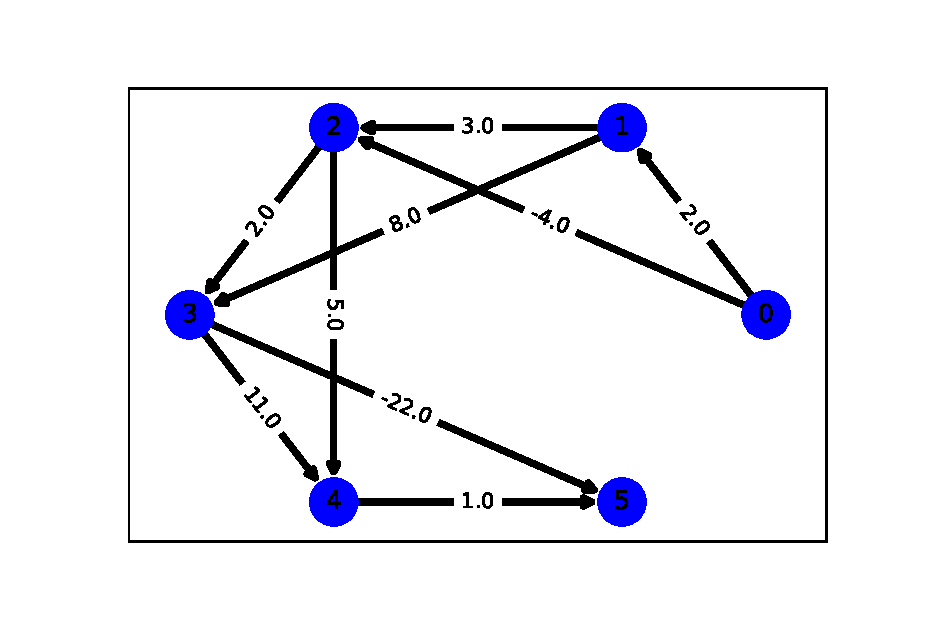
\includegraphics[scale = 0.35]{ejemplo3.eps}
\caption{grafo 1}
\label{fig:1}
\end{minipage}
\hspace{0.5 cm}
\begin{minipage}[b]{0.4\linewidth}
  \centering
  \includegraphics[scale = 0.35]{ejemplo7.eps}
  \caption{grafo 2}
  \label{fig:2}
\end{minipage}
\end{figure}

En ambos grafos se utilizó un archivo .txt de los caminos que los conectan, estos mismos se pueden encontrar en el mismo repositorio antes mencionado.

El algoritmo solo acepta nodos con nombres numéricos por lo cual los grafos 1 y 2 se modificaron en el archivo .txt de manera que a = 1, b = 2 ... etc.

Se corrieron otros ejemplos obteniendo los arcos de sus cortes mínimos.

\section{Resultados}
En ambos grafos se obtuvo un resultado de flujo máximo de 4, obteniendo la solución correcta y además se obtuvieron los arcos de mínimo corte.

\section{Mejoras}
La lectura de archivos no es la más eficiente, pero personalmente fue la más práctica ya que logramos tener la capacidad y las direcciones en un solo archivo, sin embargo espero mejorar ese aspecto; otro aspecto a mejorar sería que solo acepta como nodo inicial el nodo 1 y solo acepta nombres numéricos, se agregó un modulo en el cual puedes ingresar los datos de la matriz adyacente.

\section{Alternativa Networkx}
Una de las alternativas más atractivas es el uso de la biblioteca Networkx, la cual nos permite el uso de un comando que es \textit{\text{maximum\_flow\_value}} el cual nos pide tres elementos (G,s,t) siendo G el grafo previamente definido con comando y sintaxis de la misma biblioteca, s que sería el nodo de inicio y t que representa el nodo final; anteriormente ya había mencionado lo práctico que es esta biblioteca ya que una vez que se defina el grafo podemos dibujarlo o inclusive aplicarle alguno de los algoritmos disponibles.

Un dato curioso es que la biblioteca de Networkx no reporta los arcos de mínimo corte solo reporta el total de los cortes mínimos.

\subsection{Ejemplo Networkx}
En la siguiente figura se muestra el ejemplo que se utilizó para la biblioteca Networkx.

\begin{figure}[h!t]
  \centering
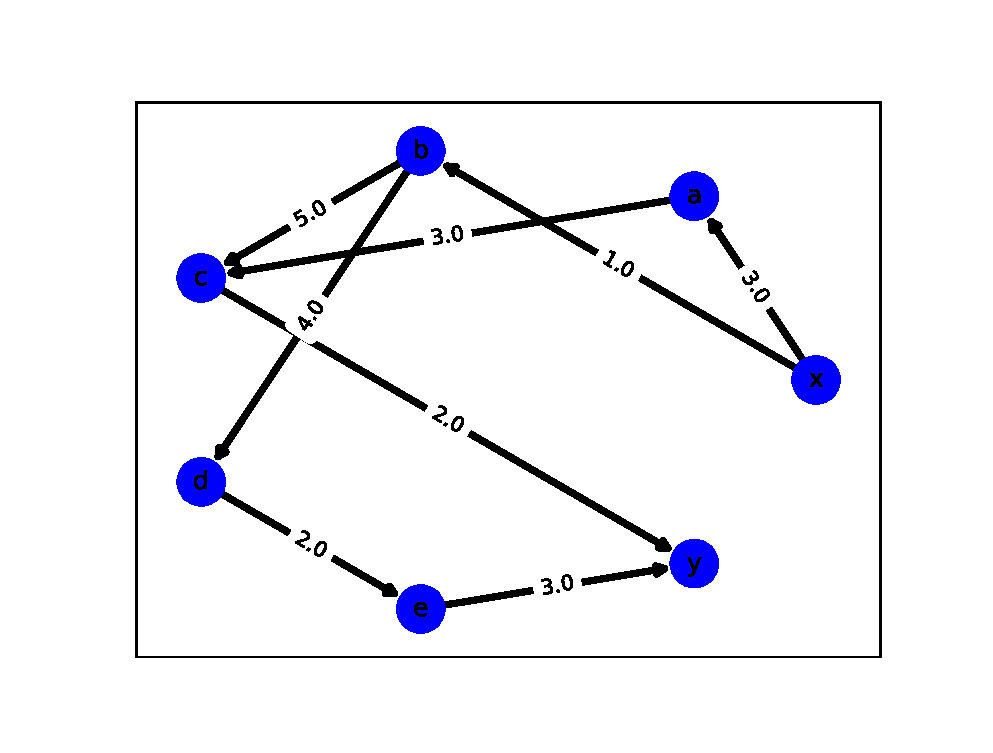
\includegraphics[scale = 0.5]{ejemplo9.eps}
\caption{Grafo para Networkx}
\label{fig:3}  
\end{figure}

\subsection{Implementación}
Al ser una biblioteca ya definida realmente no se programó demasiado, sin embargo en el mismo código se dejo una condición donde podemos obtener la ejecución de la biblioteca con el mismo archivo seleccionado.

\subsection{Resultados}
El resultado obtenido fue de 3, resultado que resulta ser correcto, además se utilizó para verificar los ejemplos anteriores.

\vspace{1 cm}

Se utilizaron los siguientes libros:
\cite{chun2001core}
\cite{van1991guia}
\cite{van2017tutorial}, lo cuales se usaron de consulta para python.
\bibliography{biblio}
\bibliographystyle{alpha}



\end{document}

